\documentclass{article}
\usepackage[utf8]{inputenc}
\usepackage{graphicx}
\graphicspath{ {Desktop/} }
\usepackage{hyperref}
\usepackage{tikz}
\usetikzlibrary{positioning}
\hypersetup{
    colorlinks=true,
    linkcolor=blue,
    filecolor=magenta,      
    urlcolor=cyan,
}

\title{\Huge \textbf{Map Reduce}}
\author{\large{Adib Alwani, Bhavin Vora, Rachit Puri, Rushikesh Badami}}
\date{April 2016}

\begin{document}

\maketitle

\section{Introduction}

This Map Reduce system like Apache Hadoop M-R framework allows for distributed processing of large data sets across clusters of computers using simple programming models. It is designed to scale up from single servers to thousands of machines, each offering local computation and storage. These clusters run on AWS EC2 instances using Amazon Linux AMI (64-Bit) machines. There is no restriction to the number of instances that user can run. By default, we run t2.medium instances. 

\section{Assumptions}

\begin{enumerate}
    \item We expect the jar name to be same as the main class name.
    
    \item After every job completion we expect client to delete partition and output folder from S3 bucket.
    
    \item All classes import edu.neu.hadoop.mapreduce.Context
    
    \item All classes import edu.neu.hadoop.mapreduce.* instead of org.apache.hadoop.mapreduce.*
    
    \item All the programs of team Puri\_Alwani are tested. 
    
\end{enumerate}


\section{Implementation}

We had to implement a system similar to hadoop map reduce system. This system will achieve the same functionality as hadoop. The system is designed to work in two modes, pseudo distributed mode and 
fully distributed mode. The goal of our project is to understand how hadoop map reduce works and try to implement a system which works similar to hadoop map reduce or better than hadoop map reduce.

\section{Design}

\subsection{Overview}

Following is the brief step-by-step process of our design for Pseudo mode:

\begin{enumerate}
    \item We have a master which spawns multiple mapper to read data.
    \item The data is shuffled and sorted and spilled to disk as a serialized object.
    \item Data from mapper is spilled on to the disk in the partition created by our partitioner.
    \item We have multiple reducer threads which are then spawned to complete the reduce task.
    \item These threads read data from respective partitions and perform the reduce task.
    \item We finally merge the data spilled from the reducer into single file and then write the data to the users local system.
\end{enumerate}

Following is the brief step-by-step process of our design for fully distributed mode:

\begin{enumerate}
    \item We spawn a Master, Worker nodes as EC2 instances.
    
    \item Master receives a list of worker nodes which will work as mappers and reducers to work in a parallel distributed system for processing output.

    \item Master will assign a part of input data to each worker node to process the data.

    \item  Each worker node processes the data (i.e. it performs its mapper and reducer tasks and writes the data to partition on s3.

    \item  Then we merge the processed data and the client can download this data from s3.

    \item  For communication between worker nodes and  master we have used socket communication. Master sends and receives data on 10000 and 10001 ports respectively. Mappers and Reducers of worker nodes send and receive data on port 10000 and 10001 respectively.

    \item We have put a barrier in master which waits for all the worker nodes to finish the mapper tasks and reducer tasks assigned to them. When all worker nodes finish mapper tasks barrier is lifted and reducer task is assigned to worker nodes. Now, Master again puts the barrier and wait for reducers tasks to get finished.
    
    \item Reducer finally writes there output in S3 which client can download.

\end{enumerate}

\subsection{Start Cluster}
First, we start clusters on EC2 instances using script \textbf{ ./start-cluster [Number of instances]}. By default, we run t2.medium machines and wait till all the instances are up. We assign one node as Master and (number of instances - 1) as our worker nodes. We save DNS information of all instances locally in a instance-dns file. It takes 1min 45sec to start cluster of 4 nodes.

\subsection{Setup Cluster}
Once clusters are up, we transfer hadoop.jar, Makefile, instance-dns file, and AWS credentials to all the worker nodes. Now, all the nodes can access S3 bucket and has information about DNS of all the other nodes in a cluster.\\
After basic setup is done, we run \textbf{runNodes.sh} script that further runs Master and Worker nodes. A Master node opens up ports {9999, 10000, 10001} and starts listening for a Job request on port 9999 from a Client and response from worker nodes on port 10000 and 10001. Where as, worker nodes opens up ports {10000, 10001} that listens for a request from Master to run Mapper and Reducer respectively.\\

\subsection{Job Submission}
Client runs the job on our cluster using script \textbf{./my-mapreduce Job.jar input-path output-path}. Internally, my-mapreduce has multiple scripts that perform following functions.
\begin{enumerate}
    \item \textbf{chunk.py} analyse the input path and create files S3data[worker node].txt that contains information about which file needs to be downloaded from S3 by each worker node.
    \item \textbf{copyClassFiles.py} extracts the jar file and copy classFiles along with S3data information to respective worker nodes.
    \item \textbf{copy.sh} tells each worker node to download respective input files from S3.
    \item Finally, we notify Master to start the Job.
\end{enumerate}

\includegraphics{design}
\pagebreak

\subsection{Mapper Phase}
In Mapper Phase, Master notifies all the worker nodes to start there Mapper and Master puts a barrier on itself which waits for all the worker nodes to notify once they are done with there mapper task. We have 100k buffer for each worker node which spills data into disk once buffer is full. Now, each worker node reads input data and writes data locally into partition folder based on hashing. So, partition folder has further sub-directory numbered as {0,1,2 ...} that contains files for each reducers. Once mapper has read all the input data, it then writes all the partition data into S3 folder and notify Master about it's completion. Similarly, all worker nodes perform this operation and notifies Master.

\subsection{Reducer Phase}
When all the worker nodes have notified about their mapper phase completion, then Master lifts its barrier and notifies all the worker nodes to start their reducer phase and puts the barrier again. Each worker node is listening at port 10001 for a request from Master and starts reducer task once notified. Each node now downloads the respective partition folder from S3 locally and starts its reducer task. After processing all the data, reducer finally writes to clients S3 output folder as part-00000, part-00001 based on reducer number and notifies Master about reducer task completion.

\subsection{Job Completion}
Once Master has been notified about reducer completion from all the worker nodes, it then lifts its barrier and is ready to process another Job request from a Client. 

\section{Problems Faced}
\begin{enumerate}

    \item Transferring input data from S3 bucket to EC2 instances - EC2 instance was not accepting the AWS credentials, we had to write system calls "check call" using python to resolve the issue. To accomplish this we copied our credential files to our EC2 instances and automated the process.

    \item Connection Refused Error - When we setup the clusters and ssh each EC2 instance to transfer the data often the request to connect was refused leading to exceptions in the start.sh file and abrupt termination of program. We had to write a system call "check call" in python to solve this issue.

    \item Communication between EC2 instances - We were not able to establish communication between EC2 instances. So we tried pinging the instances locally to check whether the servers were up on the corresponding port, it turned out that the port mapping was wrong.

\end{enumerate}

\section{Contribution}

\begin{itemize}
    \item \textbf{Design}: Adib Alwani, Rachit Puri, Bhavin Vora, Rushikesh Badami
    \item \textbf{Start and Stop Cluster}: Adib Alwani, Rachit Puri, Bhavin Vora, Rushikesh Badami
    \item \textbf{Mapper Phase} Adib Alwani
    \item \textbf{Reducer Phase} Adib Alwani
    \item \textbf{Network Manager} Adib Alwani, Bhavin Vora
    \item \textbf{Partition} Adib Alwani, Rachit Puri, Bhavin Vora, Rushikesh Badami
    \item \textbf{Merge} Adib Alwani, Rachit Puri, Bhavin Vora, Rushikesh Badami
    \item \textbf{File system} Adib Alwani, Rushikesh Badami
    \item \textbf{io} Adib Alwani, Rachit Puri, Bhavin Vora, Rushikesh Badami
    \item \textbf{Configuration} Adib Alwani, Rachit Puri
    \item \textbf{Scripts} Adib Alwani, Rachit Puri, Bhavin Vora, Rushikesh Badami
\end{itemize}

\section{Performance}

\begin{table}[ht]
    \caption{Execution Time}
    \centering
    \begin{tabular}{c|c|c}
    \hline \hline
    Assignment & Pseudo Time (min:sec) & EC2 Time (min:sec)\\
    \hline
    WordCount & 0:06 & 0:16\\
    WordMedian & 0:05 & 0:26\\
    Assignment 2 & 1:27 & 1:11\\
    Assignment 5 & 0:14 & 2:45\\
    Assignment 7 & 8:20 & 18:20\\
    \hline
    \end{tabular}
\end{table}

\pagebreak
\section{Output}

\textbf{\large{\underline{Word Count}}}\\

\begin{table}[ht]
    \caption{Word Count}
    \centering
    \begin{tabular}{c|c}
    \hline \hline
    Word & Count\\
    \hline
'TIS &  1\\
--SAID &    1\\
Come &  1\\
Coming &    1\\
Defects, &  1\\
Edwin & 1\\
French, &   1\\
HOW &   1\\
He's &  1\\
How &   1\\
I & 7\\
I'll &  2\\
Information &   1\\
Keep &  1\\
Let &   1\\
Plain & 2\\
    \hline
    \end{tabular}
\end{table}



\textbf{\large{\underline{Word Median}}}\\

Median for Alice.txt is 4\\

\textbf{\large{\underline{Assignment A2}}}\\

\begin{table}[ht]
    \caption{Cluster Analysis}
    \centering
    \begin{tabular}{c|c|c|c}
    \hline \hline
    Carrier\_Code & month & total\_flights & average\_price\\
    \hline
AS &  Jan &  13213  &  230.1071\\ 
B6 &  Jan &  21579  &  523.6475\\ 
MQ &  Jan &  29635  & 288.2641\\
US &  Jan &  33424  & 600.1602\\
UA &  Jan &  38324  & 969.0908\\
AA &  Jan &  43971  & 530.1820\\
OO &  Jan &  47737  & 307.3462\\
EV &  Jan &  49589  & 305.6798\\
DL &  Jan &  64082  & 598.8078\\
WN &  Jan &  99553  & 159.3560\\
    \hline
    \end{tabular}
\end{table}

\pagebreak

\textbf{\large{\underline{Assignment A5}}}\\

The following is the output generated for 298.csv.gz in solution\_final:

\begin{table}[ht]
    \caption{Missed Connections}
    \centering
    \begin{tabular}{c|c|c|c|c}
    \hline \hline
    Carrier\_Code & Year & Connection & MissedConnection & Percentage\\
    \hline
OO  &   2015 &  809660 &    77082       &   9.52029\\
MQ  &   2015 &  688052  &   57960       &   8.42378\\
NK  &   2015 &  34550   &   3099        &   8.96961\\
B6  &   2015 &  225131  &   16485       &   7.3224\\
UA  &   2015 &  788657  &   49458       &   6.27117\\
AS  &   2015 &  135613  &   8052        &   5.93748\\
VX  &   2015 &  25446   &   1635        &   6.42537\\
HA  &   2015 &  91333   &   4297        &   4.70476\\
WN  &   2015 &  2326906 &   110406      &   4.74476\\
AA  &   2015 &  1746964 &   103657      &   5.93355\\
F9  &   2015 &  38548   &   4851        &   12.5843\\
EV  &   2015 &  967322  &   73814       &   7.63076\\
DL  &   2015 &  3836174 &   154285      &   4.02185\\
US  &   2015 &  937179  &   48540       &   5.17937\\
    \hline
    \end{tabular}
\end{table}

\textbf{\large{\underline{Assignment A7}}}\\

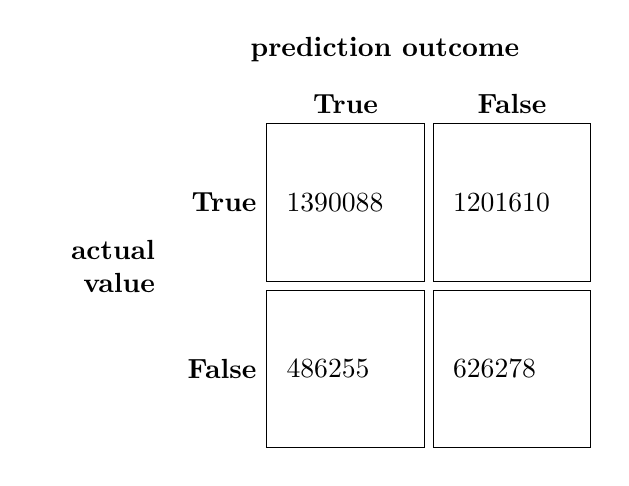
\begin{tikzpicture}[
box/.style={draw,rectangle,minimum size=2cm,text width=1.5cm,align=left}]
\matrix (conmat) [row sep=.1cm,column sep=.1cm] {
\node (tpos) [box,
    label=left:\( \mathbf{True} \),
    label=above:\( \mathbf{True} \),
    ] {1390088};
&
\node (fneg) [box,
    label=above:\textbf{False}] {1201610};
\\
\node (fpos) [box,
    label=left:\( \mathbf{False} \)] {486255};
&
\node (tneg) [box] {626278};
\\
};
\node [left=.05cm of conmat,text width=1.5cm,align=right] {\textbf{actual \\ value}};
\node [above=.05cm of conmat] {\textbf{prediction outcome}};
\end{tikzpicture}\\


Accuracy : (True\_True + False\_False)/Total = 54.4341322126

\section{Conclusion}

\begin{enumerate}
    \item Our start cluster takes less time than actual hadoop because we are running it on EC2 cluster where as hadoop runs our job on EMR cluster which might take time depending upon our job position in scheduler as well as traffic at that moment. 
    \item We are analysing the input data at Client side and decide which worker node will work on which files where as in hadoop, when job is submitted Master breaks down the input data and assign it to worker nodes.
    \item We are splitting the input files into equal partition and not considering further splitting of individual file.
    \item If any reducer goes down and Master has not lifted its barrier then system results into a deadlock condition and client has to restart the cluster manually.
\end{enumerate}



\section{References}

\begin{enumerate}
    \item \href{https://hadoop.apache.org/docs/stable/api/}{Apache Hadoop API}
    \item \href{https://github.com/apache/hadoop}{Hadoop GitHub source code}
    \item \href{https://examples.javacodegeeks.com/core-java/reflection/java-reflection-example/}{Reflection Java example}
\end{enumerate}

\end{document}
